\section{Requirement Discovery Tree}
\label{blRDT}
The requirement discovery process begins with the restatement of the mission need statement. From there, the top level requirements and their derivatives can be analysed.
\subsection{Mission Need Statement}
\label{dsePPMNS}
Demonstrate that a satellite constellation, consisting of a single emitter and several receivers, will perform superior (in terms of cost and lifetime) to existing spaceborne laser altimetry systems.
\subsection{Requirement Discovery}
\label{blReqDesq}
From the \ac{MNS} in section \ref{dsePPMNS}, it possible to deduce the top level requirements of this project. They are as follows:
\begin{itemize}
	\item Cost budget below existing spaceborne laser altimetry systems.
	\item Lifetime above existing spaceborne laser altimetry systems.
\end{itemize}
Furthermore, several more requirements were provided by the principle tutor:
\begin{itemize}
	\item Mass budget below or equal to existing spaceborne laser altimetry systems.
	\item No scanner may be used.
\end{itemize}
The last requirement is mainly considered as a pure constraint. The constellation should be designed as a collection of pointing devices.

The other three top requirements have been put in respective Requirement Discovery Trees (RDT) in appendix \ref{reqdisctree}. The following sections contain a brief discussion of each of these breakdowns.
\subsubsection{Cost Budget Requirement}
\label{blCBR}
The cost budget requirement is mainly based on the analysis of the costs of current laser altimetry systems. As a reference point, the estimated budget of the ICESat system was taken: around \$200m\cite{icesatc98a}. From hereon, the cost requirement was broken down into three main parts: payload, bus and \emph{wraps}. 

The payload defines the design requirements for the emitter and the receivers. These are then further broken down into smaller considerations.

The bus requirements are those imposed on different spacecraft subsystems, excluding the payload. Only those systems that fall under the scope of the feasibility study are examined. Spacecraft structures and thermal control are taken to have a standard budget percentage and are not elaborated. Spacecraft power, data handling and \ac{ADCS} are considered to be critical design parts thus, have their requirements listed to maximum detail.

The final section - \emph{wraps}, contains non-physical factors, such as system engineering, management and product testing. Since \emph{wraps} typically account for close to 30\% of the total budget\cite{larson}, it was imperative that these systems would be accounted, yet their design was assumed to be similar to the design of current laser altimetry systems.

\subsubsection{Mass Budget Requirement}
\label{blMBR} 
The mass budget is also a very important requirement. In order to keep total mass to the minimum (to ensure a cheap and unified launch), all critical subsystems and the payload have to be examined. In this sense, the requirement discovery tree for the mass budget looks very similar to that of the cost requirement. This is because all these design choices effect both factors. Some preliminary dry mass percentages (based on statistical data\cite{larson}) have been added to the tree to illustrate a primitive order of importance.

\subsubsection{Lifetime Requirement}
\label{blLBR}
The lifetime requirement is quite crucial. From the experience of ICESat it is apparent that payload quality (especially that of the laser) plays a pivotal role. The ICESat mission provided the satellite with three lasers in the \ac{GLAS}, first of which stopped emitting pulses on operating day 37\cite{glasreview}. The Anomaly Review Board had determined that it was the manufacturing flaws in the laser diode arrays that had led to unexpected behavior of the emitter\cite{glasreview}.

\begin{wrapfigure}{l}{0.3\textwidth}
	\begin{center}
  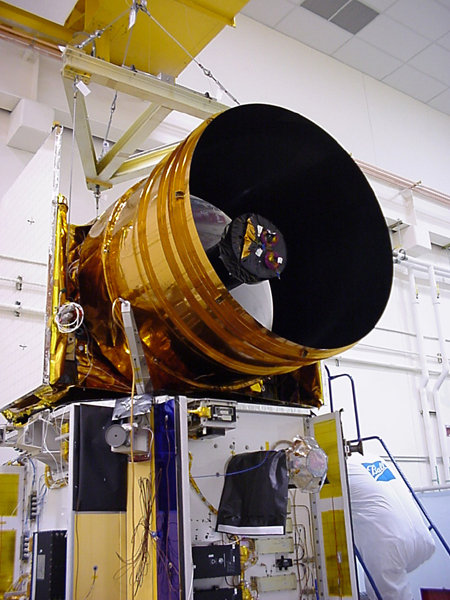
\includegraphics[width=0.3\textwidth]{chapters/img/glas.jpg}
  \end{center}
  \caption{\ac{GLAS} installed on the ICESat. \emph{http://icesat.gsfc.nasa.gov/}}
  \label{fig:glas}
\end{wrapfigure}

It is therefore required to ensure component quality and reliability in order for the mission to succeed.

Furthermore, in terms of lifetime, consideration is given to the power generation. Power source degradation will have to be carefully looked at, as the instrument without sufficient power supply will not fulfill the requirement  